%--------Experimentación
%--------Daniel Ochoa John
%--------13/10/2014
\newcolumntype{L}[1]{>{\raggedright\let\newline\\\arraybackslash\hspace{0pt}}m{#1}}
\newcolumntype{C}[1]{>{\centering\let\newline\\\arraybackslash\hspace{0pt}}m{#1}}
\newcolumntype{R}[1]{>{\raggedleft\let\newline\\\arraybackslash\hspace{0pt}}m{#1}}

\chapter{Experimentación}
\label{cap:experimentacion}

En este capítulo se tratará el experimento realizado, ejecutado bajo todo el desarrollo tecnológico descrito en los Capítulos 3 y 4, que implica la manera de probar la hipótesis que este trabajo de tesis postula. En primer lugar, se describe el experimento realizado, considerando inputs, outputs y puntos de evaluación. Luego, se caracterizan los \textit{data\textit{set}} utilizados, describiendo su dominio y cuantificando su tamaño. Finalmente, se muestran los resultados obtenidos.

\section{Descripción del experimento}

En esta sección se describe el experimento que se ha realizado para cumplir con el objetivo general de este trabajo, que es probar que existe una mejora en la eficiencia de la recomendación al contar con un mecanismo de persistencia y reutilización de las comunidades detectadas al momento de recomendar contenido a los usuarios.

Para describir el experimento, es necesario mencionar que, en el flujo de datos propuesto por RBox, al momento de generar una recomendación es posible también obtener comunidades de usuarios con intereses similares (ver Figura \ref{fig:exp-im1}). El asunto tiene que ver con persistir la existencia de las comunidades y utilizarlas como un antecedente que haga más eficiente recomendaciones posteriores, por lo que el experimento buscará evaluar si persistir las comunidades detectadas en una primera recomendación acelera o no el proceso de recomendación en ejecuciones posteriores, sobre un sistema de recomendación generado con RBox.

\begin{figure}
  \centering
  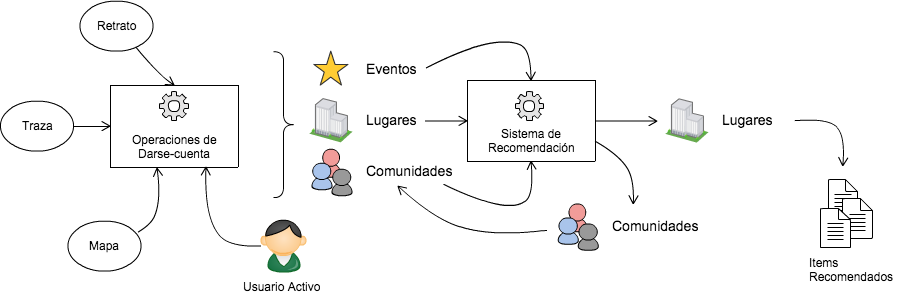
\includegraphics[scale=.5]{images/Figura5-1}
  \caption{\em Ciclo de recomendación en RBox.}
  \label{fig:exp-im1}
\end{figure}

Con este objetivo es que se ha generado un \textit{data\textit{set}} que será descrito en la sección siguiente. Sobre él se generará una recomendación de \textit{tags} considerando detección de comunidades, en tres escenarios que se detallarán más adelante. La detección de comunidades será llevada a cabo mediante los distintos algoritmos que provee el servicio, ya descrito en el Capítulo 4. Luego, se comparan los tiempos de ejecución considerando los escenarios de prueba.

\section{Caracterización de \textit{data\textit{set}}}

El \textit{data\textit{set}} que se ha utilizado para llevar a cabo el experimento ha sido obtenido a partir de la red social \textit{Twitter}. En concreto, se han generado un extractor de \textit{tweets} utilizando Ruby como lenguaje de programación. El extractor utiliza una gema llamada \textit{\textit{tweets}tream} para acceder a la Streaming API de \textit{Twitter}, permitiendo obtener el acceso a \textit{tweets} de índole público, en tiempo real. Cada uno de los \textit{tweets} es transformado a lógica 3-Ontology por el extractor y es persistido con la ayuda de un ORM\footnote{El mapeo objeto-relacional (en inglés \textit{Object Relational Mapping}, es una técnica que permite relacionar el diseño de clases de un diseño orientado a objetos, con un esquema de algún medio persistente.)} llamado Sequel\footnote{Fuentes y \textit{home} del proyecto en https://github.com/jeremyevans/sequel}.

El \textit{data\textit{set}} corresponde a una extracción dirigida de \textit{tweets}, orientado a la Copa Mundial de la Fifa Brasil 2014, para la que \textit{Twitter} ha promovido el uso de hash\textit{tags} particulares para cada país, como muestra la Tabla \ref{tab:exp-tab01}. Se ha hecho seguimiento a los comentarios que tengan que ver con los equipos sudamericanos que participan en la competición. La cuantificación de este \textit{data\textit{set}} se puede apreciar en la Tabla \ref{tab:exp-tab02}.  De cada uno de los \textit{tweets}, interesa saber de las siguientes interacciones:

\begin{enumerate}[I]
  \item \textbf{\textit{Mentioning}:} es el acto de referencia explícita, en un tweet, a un usuario. Denota un mensaje directo hacia otro usuario o una invitación a compartir una conversación respecto a un tema.
  \item \textbf{\textit{Tagging}:} es el acto de resaltar un concepto del mensaje utilizando un \textit{hashtag}. Generalmente, marca un tópico relevante que conlleva un interés particular del usuario, que motiva y fundamenta el contenido que ha compartido en la red social.
  \item \textbf{\textit{Replying}:} es el acto de replicar con un tweet la aseveración, comentario o mención de otro usuario.
\end{enumerate}

\begin{table}[H]
  \begin{center}
    \caption{Hash\textit{tags} particulares de cada país durante la copa mundial de la FIFA en \textit{Twitter}.}
    \label{tab:exp-tab01}
      \begin{tabular}{|L{4cm}|L{4cm}|}
        \hline
        \textbf{\textit{Hashtag}} & \textbf{País}\\ \hline
         \#CHI & Chile.\\ \hline
         \#BRA & Brasil.\\ \hline
         \#ARG & Argentina.\\ \hline
         \#COL & Colombia. \\ \hline
         \#ECU & Ecuador. \\ \hline
      \end{tabular}
  \end{center}
\end{table}

\begin{table}[H]
  \begin{center}
    \caption{Cuantificación del \textit{data\textit{set}} de la copa mundial de la FIFA.}
    \label{tab:exp-tab02}
      \begin{tabular}{|L{4cm}|L{4cm}|}
        \hline
        \textbf{Medida} & \textbf{Valor}\\ \hline
         \textit{Event} & 445.342\\ \hline
         \textit{Item} & 23.739\\ \hline
         \textit{User} & 91489\\ \hline
         \textit{Tweets} & 64.120\\ \hline
         \textit{Mentioning} & 92.519\\ \hline
         \textit{Tagging} & 349.577\\ \hline
         \textit{Replying} & 3.246\\ \hline
      \end{tabular}
  \end{center}
\end{table}

Como primer análisis, se considera el top 3 de usuarios que han compartido más \textit{tweets}, que incluyen menciones a otros usuarios (ver Tabla \ref{tab:exp-tab02}). Si se considera a estos usuarios, como activos, el grafo que representa sus interacciones se puede apreciar en las Figuras \ref{fig:exp-im2}, \ref{fig:exp-im3} y \ref{fig:exp-im4}, respectivamente. Si se realiza una detección de comunidades sobre el grafo de interacciones para estos usuarios, mediante, por ejemplo, del método \textit{Multilevel} (ver Capítulo 3), las comunidades detectadas pueden apreciarse en las Figuras \ref{fig:exp-im5}, \ref{fig:exp-im6} y \ref{fig:exp-im7}, respectivamente.

\begin{table}[H]
  \begin{center}
    \caption{Top 3 de usuarios con mas \textit{tweets} que consideran menciones a otros usuarios.}
    \label{tab:exp-tab02}
      \begin{tabular}{|L{4cm}|L{4cm}|}
        \hline
        \textbf{\textit{User} (Alias)} & \textbf{Nº de Menciones}\\ \hline
         539210296 (1) & 95\\ \hline
         2320149583 (2) & 85\\ \hline
         2463599637 (3)& 69\\ \hline
      \end{tabular}
  \end{center}
\end{table}

\begin{figure}
  \centering
  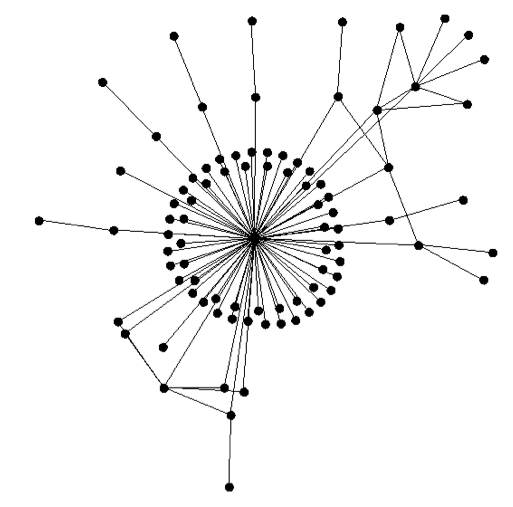
\includegraphics[scale=.7]{images/Figura5-2}
  \caption{\em Grafo de interacciones generado por el usuario 1.}
  \label{fig:exp-im2}
\end{figure}

\begin{figure}
  \centering
  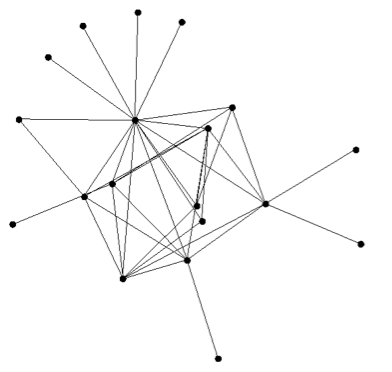
\includegraphics[scale=.7]{images/Figura5-3}
  \caption{\em Grafo de interacciones generado por el usuario 2.}
  \label{fig:exp-im3}
\end{figure}

\begin{figure}
  \centering
  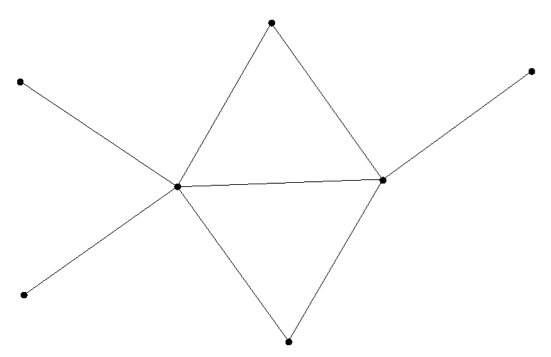
\includegraphics[scale=.7]{images/Figura5-4}
  \caption{\em Grafo de interacciones generado por el usuario 3.}
  \label{fig:exp-im4}
\end{figure}

\begin{figure}
  \centering
  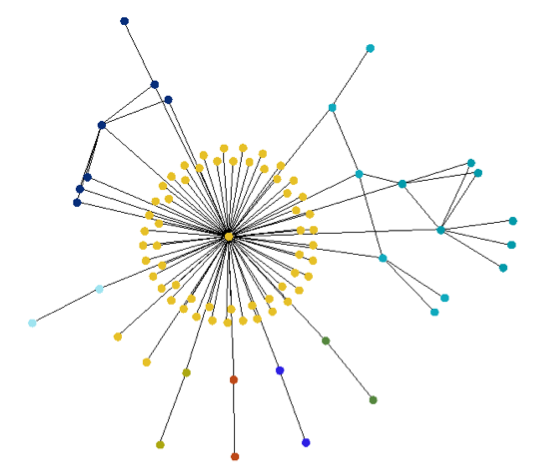
\includegraphics[scale=.7]{images/Figura5-5}
  \caption{\em Comunidades detectadas en base al grafo de interacciones generado por el usuario 1.}
  \label{fig:exp-im5}
\end{figure}

\begin{figure}
  \centering
  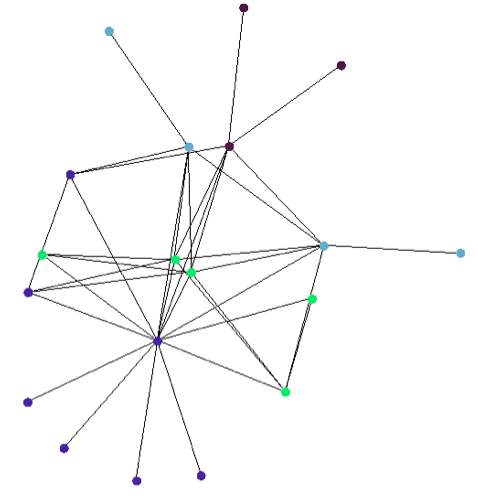
\includegraphics[scale=.7]{images/Figura5-6}
  \caption{\em Comunidades detectadas en base al grafo de interacciones generado por el usuario 2.}
  \label{fig:exp-im6}
\end{figure}

\begin{figure}
  \centering
  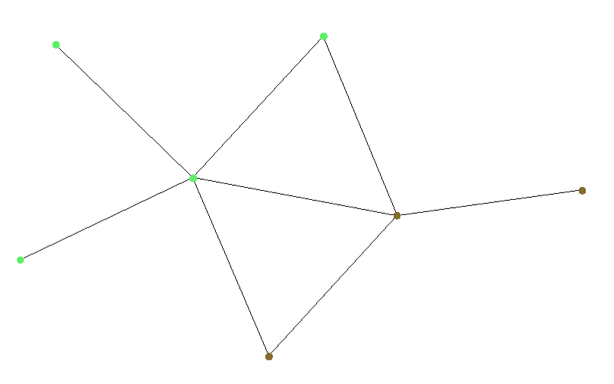
\includegraphics[scale=.7]{images/Figura5-7}
  \caption{\em Comunidades detectadas en base al grafo de interacciones generado por el usuario 3.}
  \label{fig:exp-im7}
\end{figure}

\section{Resultados}

Para experimentar con un proceso de recomendación utilizando comunidades, se ha implementado un algoritmo de recomendación de tags, cuyo objetivo es retornar los top N \textit{tags} con mayor ocurrencia en una comunidad. Para generar las comunidades, se considera el evento \textit{Mentioning}, se han omitido los registros que consideran a menos de diez menciones hacia otros usuarios para eliminar la generación de comunidades pequeñas. La distribución de \textit{mentions} del \textit{dataset}, por rango, se puede apreciar en la Tabla \ref{tab:exp-tab03}.

De cada uno de los rangos se han seleccionado aleatoriamente dos usuarios, con el objetivo de analizar los tiempos requeridos para obtener una recomendación, considerando el mecanismo de \textit{community cache} como eje al momento de persistir las comunidades que ellos generan mediante sus interacciones en la red social. 

Los escenarios de prueba son diseñados para simular el comportamiento de la \textit{community cache} y todos tienen en consideración diez iteraciones, utilizando tres métodos de detección de comunidades, \textit{Multilevel}, \textit{LeadingEigenvector} e \textit{Infomap}. Las consideraciones particulares de los escenarios tienen relación con el estado inicial del medio persistente, la estrategia de caché y el estado final del medio persistente, estos son:

\begin{enumerate}
	\item \textbf{Escenario 1 (E1)}: Considera un medio persistente inicial sin comunidades, la estrategia de persistencia es mediante el primer nivel de \textit{community cache} y al final de cada ciclo de iteraciones, el medio persistente es reiniciado.
	\item \textbf{Escenario 2 (E2)}: Considera un medio persistente inicial sin comunidades, la estrategia de persistencia es mediante el segundo nivel de \textit{community cache} y al final de cada ciclo de iteraciones, el medio persistente es reiniciado.
	\item \textbf{Escenario 3 (E3)}: Considera un medio persistente inicial sin comunidades, la estrategia de persistencia es mediante el segundo nivel de \textit{community cache} y al final de cada ciclo de iteraciones se conserva el medio persistente.
\end{enumerate}

El experimento considera la ejecución de cada uno de los escenarios, para todos los usuarios, detectando comunidades mediante los tres métodos. La referencia de los usuarios seleccionados y sus interacciones mediante mentions se puede apreciar en la Tabla \ref{tab:exp-tab04}, se les ha asignado un alias que permitirá identificarlos de manera abreviada en los análisis venideros.

\begin{table}[H]
  \begin{center}
    \caption{Distribución de eventos \textit{mention} en el \textit{dataset}.}
    \label{tab:exp-tab03}
      \begin{tabular}{|L{4cm}|L{4cm}|}
        \hline
        \textbf{Rango} & \textbf{Menciones}\\ \hline
         [10 - 25) & 520\\ \hline
         [25 - 50) & 34\\ \hline
         [50 - 75) & 5\\ \hline
         [75 - 100) & 2\\ \hline
      \end{tabular}
  \end{center}
\end{table}

\begin{table}[H]
  \begin{center}
    \caption{Usuarios seleccionados, número de menciones y alias para experimento.}
    \label{tab:exp-tab04}
      \begin{tabular}{|L{4cm}|L{4cm}|L{4cm}|}
        \hline
        \textbf{Usuario} & \textbf{Menciones} & \textbf{Alias} \\ \hline
         1360359360 & 12 & U1\\ \hline
         577741173 & 24 & U2\\ \hline
         2544108592 & 49 & U3\\ \hline
         301461393 & 27 & U4\\ \hline
         2463599637 & 69 & U5\\ \hline
         525904011 & 54 & U6\\ \hline
         539210296 & 95 & U7\\ \hline
         2320149583 & 85 & U8\\ \hline
      \end{tabular}
  \end{center}
\end{table}

La Figura \ref{fig:exp-im8} muestra el comportamiento de los tiempos requeridos para realizar una recomendación al usuario Ui, en adelante Tr, en E1. Se puede apreciar que Tr experimenta un descenso progresivo a través de las iteraciones y en la iteración final Tr siempre es menor que en la primera iteración. Esto es ocasionado por la condición de inicialización del medio persistente, como no hay comunidades para el usuario activo, el tiempo es utilizado en detectar, persistir y relacionar comunidades. Como está activado el primer nivel de cache, no es necesario detectar comunidades en iteraciones posteriores, por lo que el tiempo de estabilización, entre la segunda iteración y la novena, es principalmente utilizado por el sistema de recomendación propiamente tal, y por la validación de caché.

\begin{figure}[H]
  \centering
  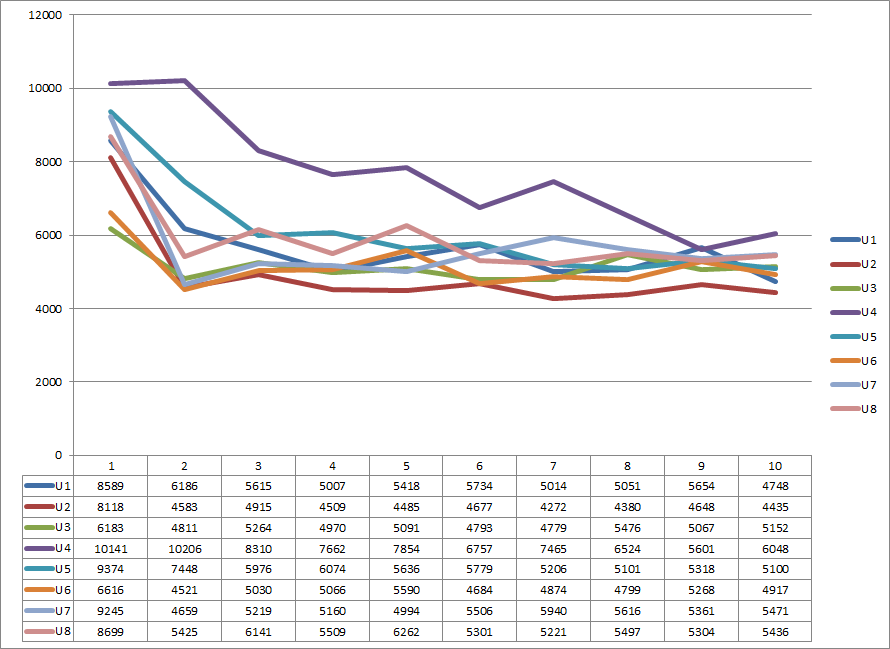
\includegraphics[scale=.7]{images/Figura5-8}
  \caption{\em Tiempos promedio (ms) requeridos para realizar una recomendación a Ui en E1.}
  \label{fig:exp-im8}
\end{figure}

La Figura \ref{fig:exp-im9} muestra el comportamiento de Tr en E2. Se puede apreciar que el descenso de Tr es muy marcado entre la primera y la segunda iteración. La estabilización de Tr parece ocurrir antes, debido a que el segundo nivel de cache controla las operaciones de persistencia innecesarias. Existen anomalías en la curva de U1 entre las iteraciones 7 y 9 debido a una sobrecarga no controlada de procesamiento mientras estaba ejecutándose la detección de comunidades por el método multilevel. Se refleja en la curva debido a la utilización de promedios para agrupar los tiempos de ejecución de los tres métodos. No obstante, la Figura \ref{fig:exp-im10} muestra el gráfico específico para U1, donde se puede apreciar explícitamente el peak de Multilevel entre las mencionadas iteraciones.

\begin{figure}[H]
  \centering
  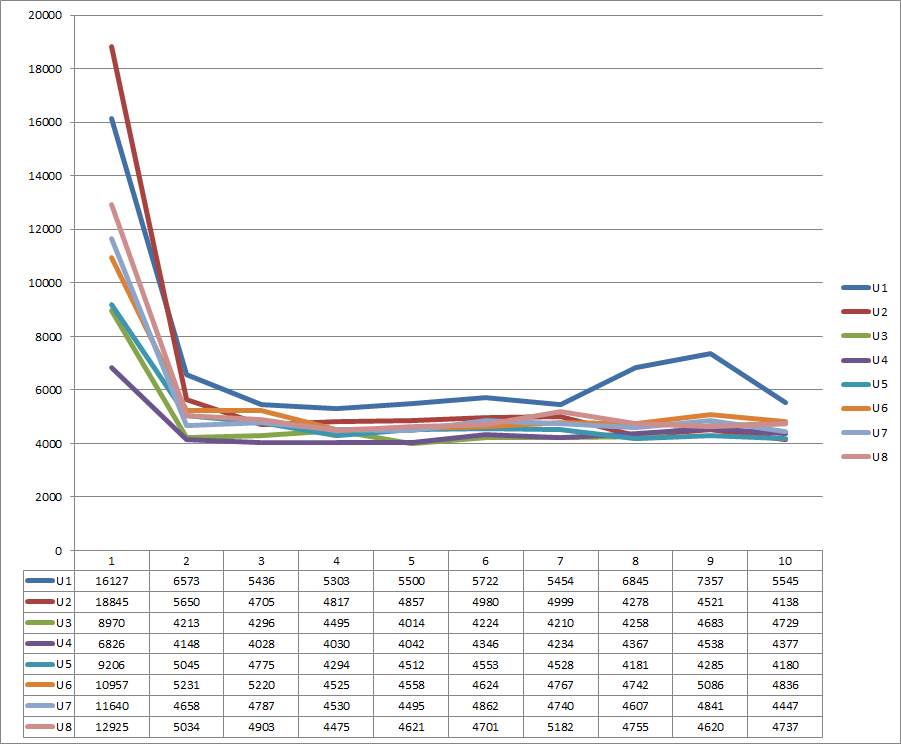
\includegraphics[scale=.7]{images/Figura5-9}
  \caption{\em Tiempos promedio (ms) requeridos para realizar una recomendación a Ui en E2.}
  \label{fig:exp-im9}
\end{figure}

\begin{figure}[H]
  \centering
  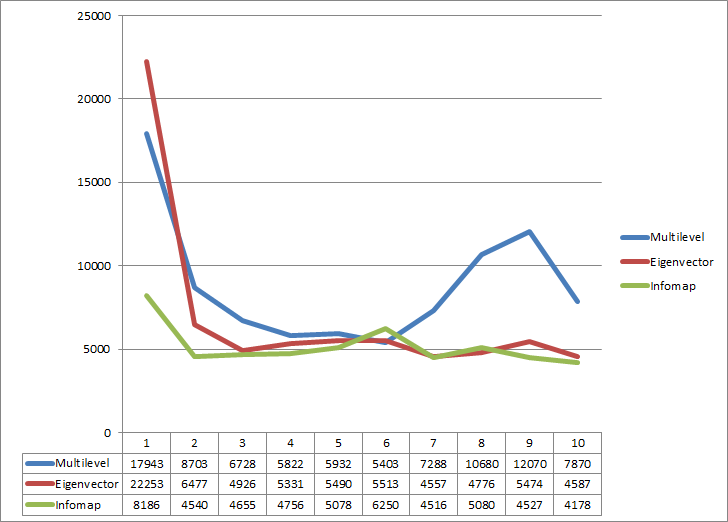
\includegraphics[scale=.7]{images/Figura5-10}
  \caption{\em Tr (ms) para U1 en E2.}
  \label{fig:exp-im10}
\end{figure}

La Figura \ref{fig:exp-im11} muestra el comportamiento de Tr en E3. La principal diferencia radica en la pequeña variación en los tiempos entre una iteración y otra. Como es la tónica, se aprecia un descenso en Tr a partir de la segunda iteración. La variación de los tiempos tiene que ver con que, como una de las condiciones de E3 es no limpiar el medio persistente al fin de cada secuencia de iteraciones, el sistema de cache tiene comunidades donde comparar y evaluar si corresponde su persistencia.

\begin{figure}[H]
  \centering
  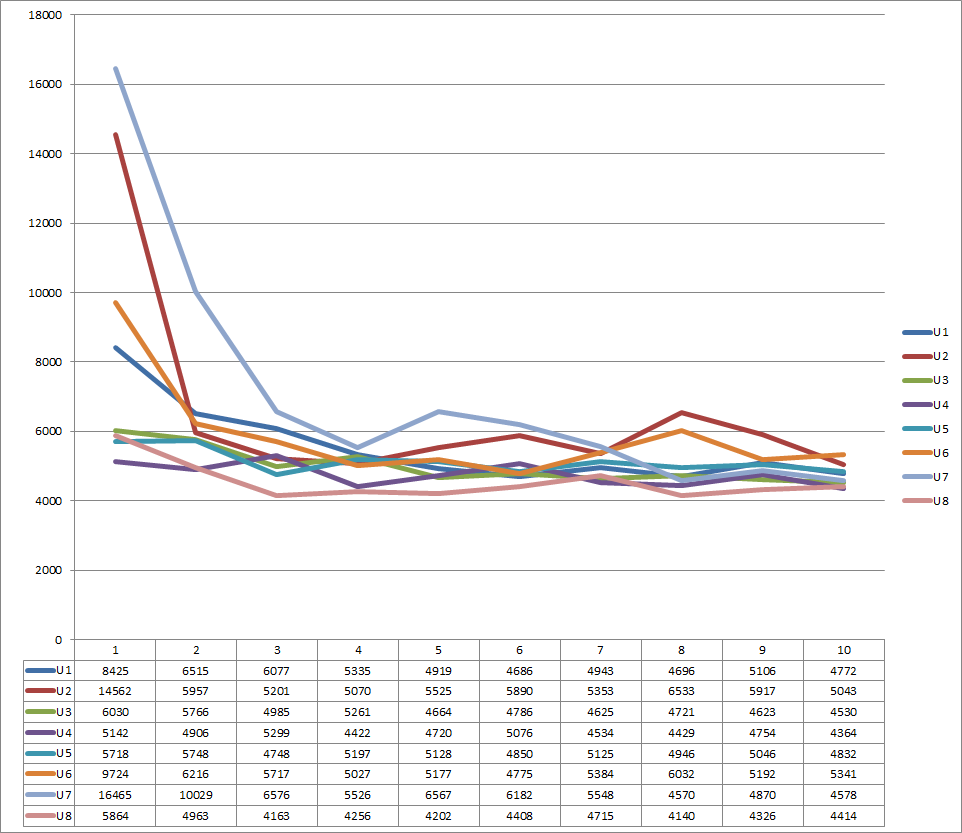
\includegraphics[scale=.7]{images/Figura5-11}
  \caption{\em Tiempos promedio (ms) requeridos para realizar una recomendación a Ui en E3.}
  \label{fig:exp-im11}
\end{figure}

La Figuras \ref{fig:exp-im12}, \ref{fig:exp-im13} y \ref{fig:exp-im14} muestran la diferencia que existe, para cada uno de los usuarios seleccionados, en Tr en tres casos: en la primera iteración (T0) , en la última (T10) y la línea del promedio (AVG), para todos los escenarios, respectivamente. Se puede apreciar que, para todos los usuarios y en todos los escenarios, siempre la primera iteración toma más Tr que la última, y más aún, que el promedio de iteraciones es menos costoso que la primera iteración. 

\begin{figure}[H]
  \centering
  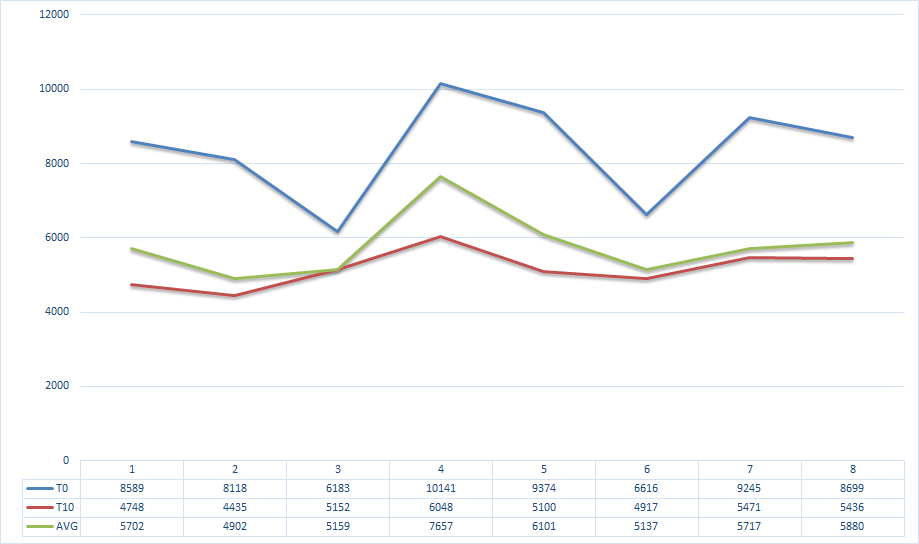
\includegraphics[scale=.7]{images/Figura5-12}
  \caption{\em Tr (ms) para T0, T10 y AVG en E1.}
  \label{fig:exp-im12}
\end{figure}

\begin{figure}[H]
  \centering
  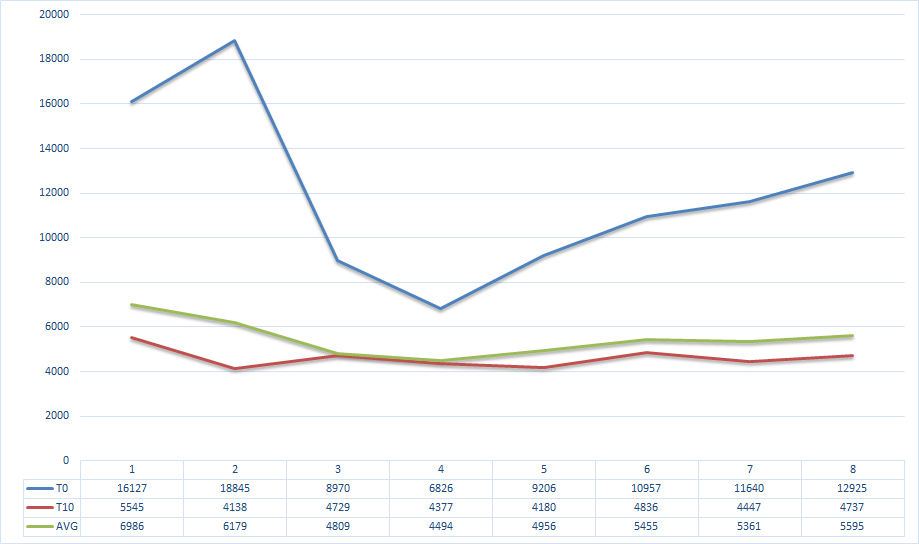
\includegraphics[scale=.7]{images/Figura5-13}
  \caption{\em Tr (ms) para T0, T10 y AVG en E2.}
  \label{fig:exp-im13}
\end{figure}

\begin{figure}[H]
  \centering
  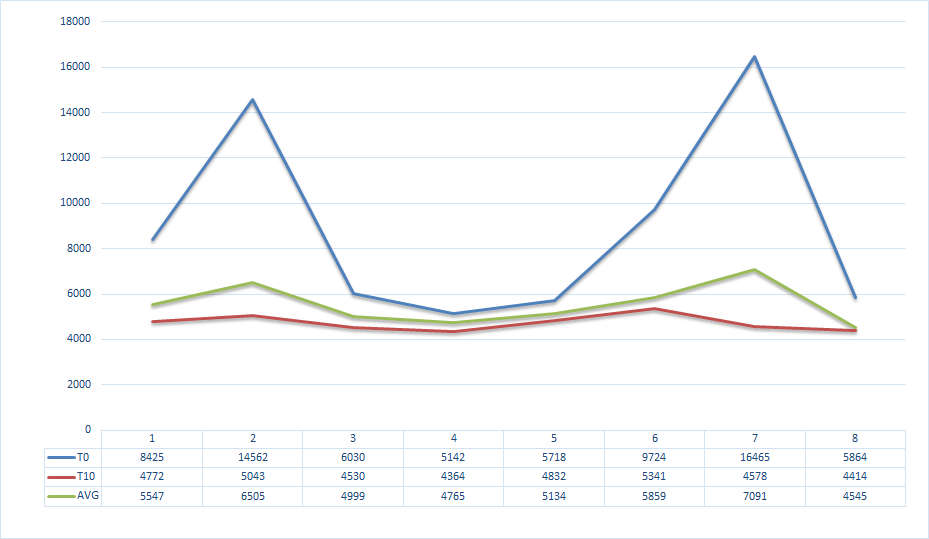
\includegraphics[scale=.7]{images/Figura5-14}
  \caption{\em Tr (ms) para T0, T10 y AVG en E3.}
  \label{fig:exp-im14}
\end{figure}

La Tabla \ref{tab:exp-tab05} muestra el análisis de varianza de factor simple (ANOVA) para Tr en E1 y E2, considerando T0 y T10 para todos los usuarios. E3 se ha dejado fuera de este análisis ya que cada iteración no es completamente independiente de otra. Se puede apreciar que F es mayor que F crit en los ambos casos, por lo que la reducción de tiempo es significativa y no dependiente de condiciones azarosas.

\begin{table}[H]
  \begin{center}
    \caption{Análisis de varianza de factor simple.}
    \label{tab:exp-tab05}
      \begin{tabular}{|L{1cm}|L{4cm}|L{4cm}|L{4cm}|}
        \hline
        \textbf{E} & \textbf{F} & \textbf{P} & \textbf{F crit} \\ \hline
         1 & 39,15251 & 2,1E-05 & 4,60011\\ \hline
         2 & 26,95112 & 0,000137 & 4,60011\\ \hline
      \end{tabular}
  \end{center}
\end{table}



\section{Resumen}

En este capítulo se ha descrito y presentado los resultados del experimento aplicado con el propósito de conseguir el objetivo general planteado en este trabajo de Tesis. En primer lugar, se ha descrito detalladamente el experimento realizado, con sus componentes y distintos escenarios. Luego, se ha caracterizado el \textit{data\textit{set}} utilizado para realizar las pruebas, describiendo el mecanismo de extracción, construcción, persistencia y cuantificación del tamaño de información contenida. Posteriormente, se han mostrado ejemplos de detección de comunidades utilizando el \textit{data\textit{set}} descrito. Finalmente, se han expuesto los resultados de la experimentación, logrando reducir el tiempo requerido para realizar una recomendación, mediante el uso del \textit{framework} y componentes descritos en los Capítulos 3 y 4.
